\documentclass{article}
    \usepackage{amssymb}
    \usepackage[utf8]{inputenc}
    \usepackage[russian]{babel}
    \usepackage[left=2cm,right=2cm,
        top=2cm,bottom=2cm,bindingoffset=0cm]{geometry}
    \usepackage{hyperref}
    \hypersetup{
        colorlinks=true,
        linkcolor=blue,
        filecolor=magenta,      
        urlcolor=cyan,
    }
  \usepackage{graphicx}
  \usepackage{booktabs}
  \graphicspath{{pictures/}}
  \DeclareGraphicsExtensions{.pdf,.png,.jpg}
\usepackage{subcaption}
%\captionsetup{compatibility=false}

\begin{document}
\begin{center}{\hugeОтчет по дипломной работе за неделю\\}\end{center}
Дата: 11.3.2021\\
Научные руководители: Герасимов С.В., Мещеряков А.В.\\
Студент: Немешаева Алиса\\
Курс: 4\\

\renewcommand{\labelitemi}{$\blacksquare$}
\renewcommand\labelitemii{$\square$}
\begin{enumerate}
    \item Добавлена иллюстрация модели Unet для статьи. 
        ~\ref{Fig:Unet}{}\\
    \item Для сравнения качества моделей был добавлен каталог Abell. Это каталог с 4073 скоплениями 
        галактик, он был первым подобным каталогом в истории. Он был составлен вручную по данным 
        оптического обзора POSS.\\
    \item Проведено сравнение отклика итоговых каталогов по Abell.
        ~\ref{Fig:Recall}{}\\
    \item Перестроен график отклика для всех эпох на восточной валидационной области.
        ~\ref{Fig:Epoch}{}\\
\end{enumerate}




\begin{figure}[h]
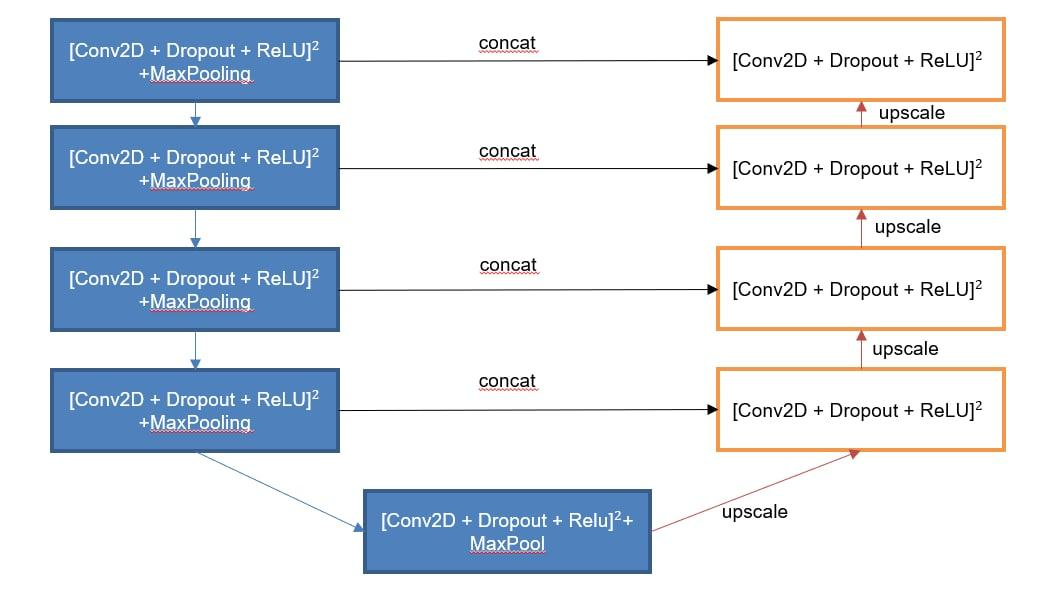
\includegraphics[width=0.8\linewidth]{unet}
\caption{Схема модели Unet}
\label{Fig:Unet}
\end{figure}
\begin{figure}[h]
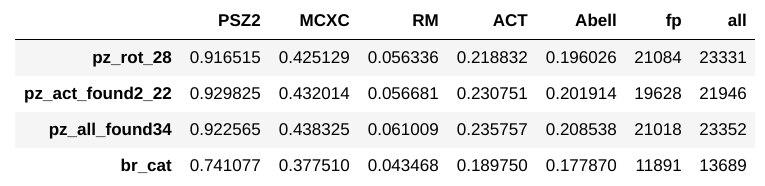
\includegraphics[width=0.8\linewidth]{recall}
\caption{Сравнение откликов наилучших каталогов}
\label{Fig:Recall}
\end{figure}

\begin{figure}[h]
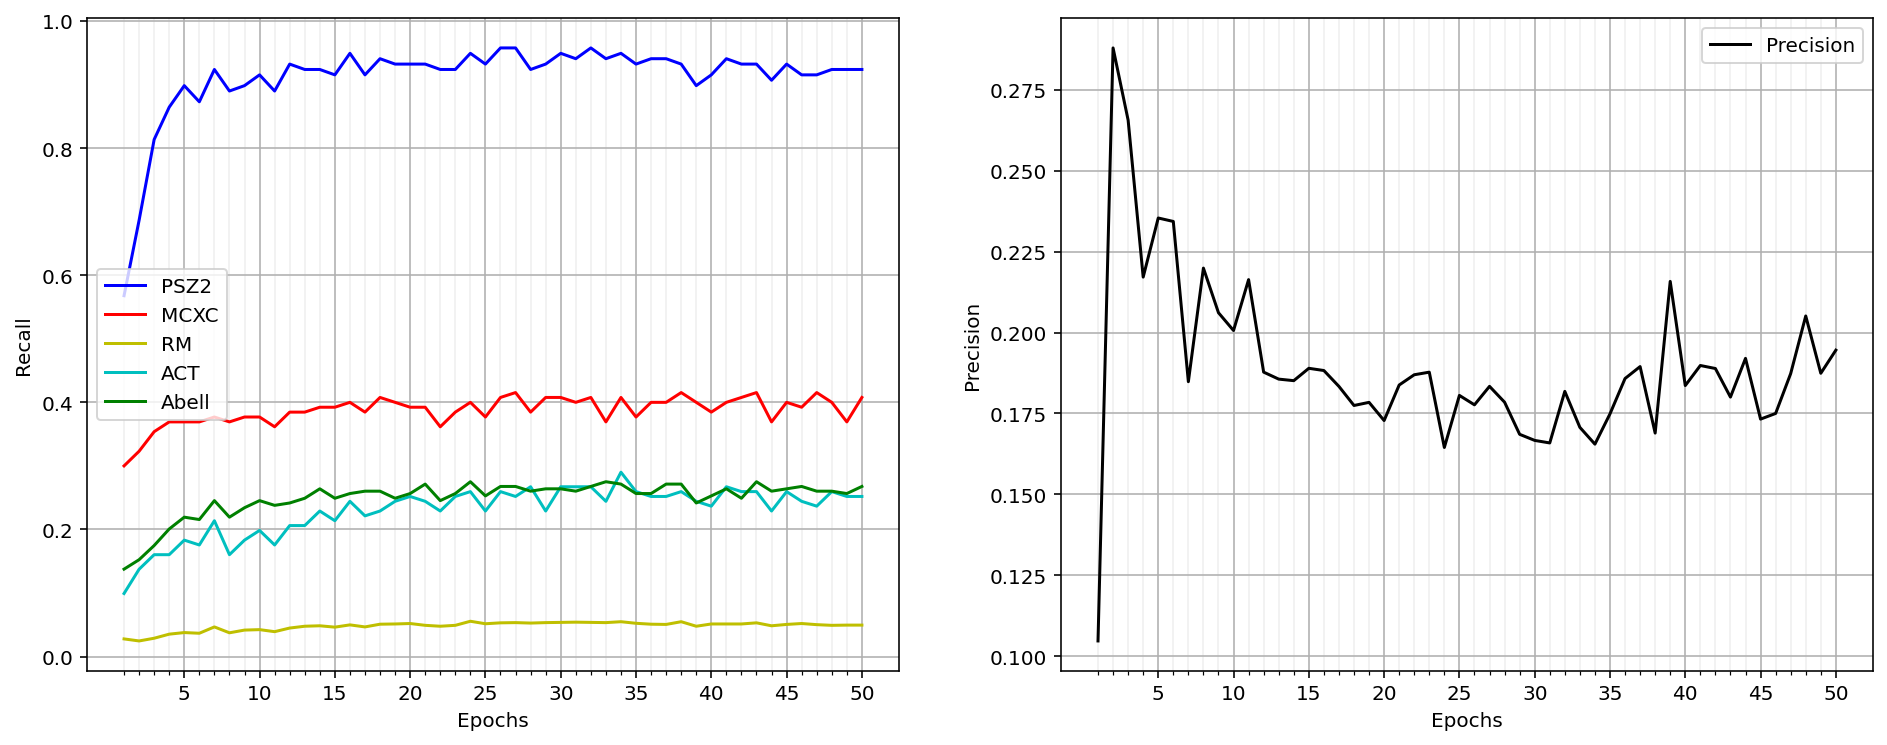
\includegraphics[width=0.8\linewidth]{recall2epoch}
\caption{Отклик (слева) и точность (справа) для каждой эпохи на тестовой области для лучшей модели.}
\label{Fig:Recall}
\end{figure}

Отчет согласован с научным руководителем.\\
Общее количество строк кода за эту неделю: 199\\
\href{https://github.com/rt2122/data-segmentation-2}{Репозиторий}\\ 
\end{document}
